\chapter{Quantifying MGXS Approximations}
\label{chap:biases}

This chapter verifies the accuracy of the data pipeline used to compute multi-group cross sections with OpenMC for use in OpenMOC. A series of case studies was devised to systematically quantify biases inherent to the energy condensation and spatial homogenization process in multi-group transport theory. The results from this chapter underline the complex interactions between discretizations in energy, space and angle. Various case studies of each of these variables are presented which quantify the resulting magnitude of the bias induced between continuous energy Monte Carlo and multi-group deterministic calculations. The results in this chapter illustrate the loss in accuracy resulting from scalar flux-weighted \ac{MGXS} and highlight the need for models of the angular dependency in \ac{MGXS} for fine-mesh neutron transport codes.


%%%%%%%%%%%%%%%%%%%%%%%%%%%%%%%%%%%%%%%%%%%%%%%%%%%%%%%%%%%%%%%%%%%%%%%%%%%%%%%%
\section{Case Studies}
\label{sec:chap4-case-studies}

This chapter investigates the loss in accuracy resulting from approximations made in both the \ac{MOC} equations as well as the \ac{MGXS} generation scheme with OpenMC. The approximation errors are quantified for a variety of geometric and material configurations. In each case, the bias $\Delta\rho$ compares the eigenvalue $k_{eff}^{OpenMOC}$ computed with \ac{MGXS} in OpenMOC to that of the reference eigenvalue $k_{eff}^{OpenMC}$ computed with continuous energy cross sections in OpenMC in units of \ac{PCM}:

\begin{equation}
\label{eqn:chap4-delta-rho}
\Delta\rho = \left(k_{eff}^{OpenMOC} - k_{eff}^{OpenMC}\right) \times 1E5
\end{equation}

\begin{itemize}[noitemsep]
  \item need to highlight sources of approximation error that are wrapped up in $\Delta\rho$
  \item highlight need for simple benchmarks to isolate errors
  \item mention cancellation of error
\end{itemize}

In each case study, the role of angular discretization in \ac{MOC} is quantified through convergence studies of the number of azimuthal angles and the track spacing used in the deterministic calculations. The effects of energy discretization are analyzed for \ac{MGXS} tallied in the CASMO~\cite{rhodes2006casmo} energy group structures ranging from 1 -- 70 groups (see~\ref{app:energy-groups}). For each of the case studies with heterogeneous geometries, the spatial domain is discretized in OpenMOC's \ac{FSR} mesh with constant-by-material \ac{MGXS} to quantify the interaction between the energy and spatial approximations. Spatial discretization studies show the impact of tallying \ac{MGXS} in each of the \ac{FSR}s used in the discretized OpenMOC geometry. Finally, \ac{MGXS} libraries were tallied using OpenMC's ``iso-in-lab'' feature to quantify the impact of the isotropic in lab scattering approximation used in OpenMOC. Inter-pin spatial self-shielding effects are not treated here as they are studied in detail in subsequent Chapters.

%%%%%%%%%%%%%%%%%%%%%%%%%%%%
\subsection{Homogeneous Infinite Medium}
\label{subsec:chap4-inf-medium}

An initial case study was performed for a homogeneous infinite medium problem. The isotopic composition of the infinite medium was constructed to mimic that of a homogenized \ac{PWR} pin cell and is described in Table~\ref{table:chap2-inf-med-isotopes}. No approximation is made in the multi-group formulation of the transport equation in the case of homogeneous infinite media. As a result, neutron balance should be exactly preserved within numerical precision in deterministic calculations with \ac{MGXS} computed in any energy group structure, assuming the tallies used to compute \ac{MGXS} are sufficiently converged.

\begin{table}[h!]
  \centering
  \caption{Homogeneous infinite medium isotopic composition.}
  \small
  \label{table:chap2-inf-med-isotopes} 
  \vspace{6pt}
  \begin{tabular}{c c}
  \toprule
  \multicolumn{1}{c}{\bf Nuclide} &
  \multicolumn{1}{c}{\bf Density [at/b-cm]} \\
  \midrule
  H-1 &   4.123778597552705E-2 \\
  O-16 &  2.062180312907649E-2 \\
  Zr-90 & 3.009046301354838E-3 \\
  U-235 & 1.623109453918422E-4 \\
  U-238 & 9.791980637067758E-3 \\
  \bottomrule
\end{tabular}
\end{table}

The reference eigenvalues computed with continuous energy cross sections in OpenMC are shown in Table~\ref{table:chap2-inf-med-reference} for both normal anisotropic as well as ``iso-in-lab'' scattering. As one would expect for a homogeneous infinite medium, the eigenvalues for anisotropic and ``iso-in-lab'' scattering match within statistics.  The reference calculations were computed for 100 batches of 1E8 particles per batch. The \texttt{openc.mgxs} module was used to compute 70-group libraries of $\Sigma^T_g$, $\nu\Sigma^F_g$, $\nu_s\Sigma^S_{gg'}$ and $\chi_g$ from OpenMC tallies. An installation of OpenMOC compiled with double precision floating point arithmetic was used for each deterministic simulation. In each calculation, OpenMOC was converged to a criterion of 1E-7 on the energy-integrated fission source.

\begin{table}[h!]
  \centering
  \caption{Reference $k^{OpenMC}_{\infty}$ for a homogeneous infinite medium.}
  \small
  \label{table:chap2-inf-med-reference} 
  \vspace{6pt}
  \begin{tabular}{c c}
  \toprule
  \multicolumn{1}{c}{\bf Anisotropic} &
  \multicolumn{1}{c}{\bf Isotropic in Lab} \\
  \midrule
  1.15908 $\pm$ 0.00001 & 1.15907 $\pm$ 0.00001 \\
  \bottomrule
\end{tabular}
\end{table}

Table~\ref{table:chap2-inf-med-angle} presents the bias $\Delta\rho$ between OpenMC and OpenMOC for a matrix of azimuthal angles and track spacings. The results for both normal and ``iso-in-lab'' scattering indicate consistent agreement of the eigenvalues computed by OpenMOC with OpenMC irregardless of track discretization.

\begin{table}[h!]
  \centering
  \caption[Angular discretization error for a homogeneous infinite medium]{Convergence study of the eigenvalue bias $\Delta\rho$ with varying azimuthal angle quadratures and track spacings for a homogeneous infinite medium.}
  \small
  \label{table:chap2-inf-med-angle}
  \vspace{6pt}
  \begin{tabular}{c S[table-format=2.1] S[table-format=2.1] S[table-format=2.1] c S[table-format=2.1] S[table-format=2.1] S[table-format=2.1]} 
  \toprule
  & \multicolumn{7}{c}{\boldmath $\Delta\rho$ {\bf [pcm]}} \\
  \midrule
  \multicolumn{1}{c}{\bf \# Angles} &
  \multicolumn{1}{c}{\bf 0.1 cm} & 
  \multicolumn{1}{c}{\bf 0.01 cm} & 
  \multicolumn{1}{c}{\bf 0.001 cm} &
  \multicolumn{1}{c}{} &
  \multicolumn{1}{c}{\bf 0.1 cm} & 
  \multicolumn{1}{c}{\bf 0.01 cm} & 
  \multicolumn{1}{c}{\bf 0.001 cm} \\
  \midrule
  & \multicolumn{3}{c}{\bf Anisotropic} &
  \multicolumn{1}{c}{} &
  \multicolumn{3}{c}{\bf Isotropic in Lab} \\
  \cline{2-4} \cline{6-8}
4 & 1.3 & 1.3 & 1.3 & & -0.1 & -0.1 & -0.1 \\
8 & 1.3 & 1.3 & 1.3 & & -0.1 & -0.1 & -0.1 \\
16 & 1.3 & 1.3 & 1.3 & & -0.1 & -0.1 & -0.1 \\
32 & 1.3 & 1.3 & 1.3 & & -0.1 & -0.1 & -0.1 \\
64 & 1.3 & 1.3 & 1.3 & & -0.1 & -0.1 & -0.1 \\
128 & 1.3 & 1.3 & 1.3 & & -0.1 & -0.1 & -0.1 \\
  \bottomrule
\end{tabular}
\end{table}

Table~\ref{table:chap2-inf-med-energy} presents the bias $\Delta\rho$ between OpenMC and OpenMOC for a matrix of energy group structures and \ac{FSR} spatial discretizations. The OpenMOC calculations each used 128 azimuthal angles and 0.05 cm track spacing. The eigenvalues vary slightly between energy group structures, but the small deviations are likely due to numerical roundoff error in the MOC calculation.

\begin{table}[h!]
  \centering
  \caption[Energy discretization error for a homogeneous infinite medium.]{Convergence study of the eigenvalue bias $\Delta\rho$ with varying energy groups structures for a homogeneous infinite medium.}
  \small
  \label{table:chap2-inf-med-energy} 
  \vspace{6pt}
  \begin{tabular}{c S[table-format=2.1] S[table-format=2.1]}
  \toprule
  \multicolumn{1}{c}{\textbf{\# Groups}} &
  \multicolumn{2}{c}{\boldmath $\Delta\rho$ {\bf [pcm]}} \\
  \midrule
  & \multicolumn{1}{c}{\bf Anisotropic} &
  \multicolumn{1}{c}{\bf Isotropic in Lab} \\
  \midrule
1 & -11.1 & -10.5 \\
2 & -9.5 & -7.1 \\
4 & -0.1 & -0.5 \\
8 & 0.3 & -0.0 \\
16 & -0.2 & 0.5 \\
25 & 1.8 & 0.1 \\
40 & 1.6 & 0.1 \\
70 & 1.3 & -0.1 \\
  \bottomrule
\end{tabular}
\end{table}


%%%%%%%%%%%%%%%%%%%%
\subsection{1D Slab}
\label{subsec:chap4-slab}

A simple slab model was constructed to quantify approximation errors in a 1D heterogeneous geometry with spatial self-shielding. The slab model was constructed as an ``equivalent'' 1D model to the 1.6\% enriched UO$_2$ \ac{PWR} fuel pin in the \ac{BEAVRS} \ac{PWR} model~\cite{horelik2013beavrs}. The geometric configuration of UO$_2$ fuel, zirconium clad and water moderator is illustrated in Figure~\ref{fig:chap4-slab} and the dimensions for each material zone are shown in Table~\ref{table:chap2-slab-widths}. The width of each spatial region corresponds to the radius of the region in the corresponding 2D fuel pin in order to preserve the mean chord length across each material. Reflective boundary conditions were applied to both left and right edges in the geometry. The isotopic composition of each material in the slab is identical to the \ac{BEAVRS} fuel pin and is itemized in Table~\ref{table:chap2-slab-isotopes}. 

\begin{figure}[h!]
\begin{subfigure}{\textwidth}
  \centering
  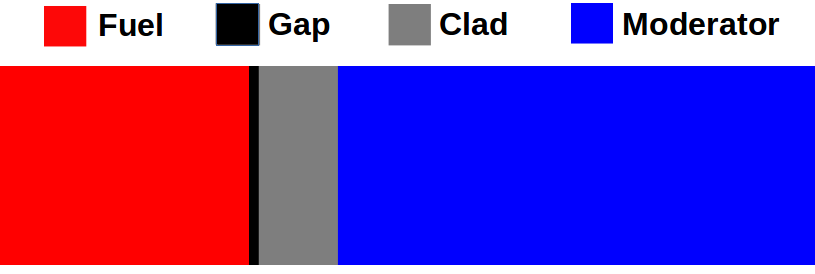
\includegraphics[width=0.7\linewidth]{figures/biases/slab/slab-simple-labels}
  \caption{}
\end{subfigure} \\
\begin{subfigure}{\textwidth}
  \centering
  
\includegraphics[width=0.7\linewidth]{figures/biases/slab/slab-8x}
  \caption{}
\end{subfigure}
\caption[1D slab materials and geometry]{A 1D slab with fuel, clad and moderator (a). Linearly-spaced tally zones were defined in each material in OpenMC and as \ac{FSR}s in OpenMOC (b).}
\label{fig:chap4-slab}
\end{figure}

\begin{table}[h!]
  \centering
  \caption{1D slab dimensions.}
  \small
  \label{table:chap2-slab-widths} 
  \vspace{6pt}
  \begin{tabular}{l c}
  \toprule
  \multicolumn{1}{c}{\bf Material} &
  \multicolumn{1}{c}{\bf Width [cm]} \\
  \midrule
  Fuel &  0.39218 \\
  Gap &   0.00787 \\
  Clad &  0.05715 \\
  Water & 0.17272 \\
  \bottomrule
\end{tabular}
\end{table}

\begin{table}[h!]
  \centering
  \caption{1D slab isotopic composition.}
  \small
  \label{table:chap2-slab-isotopes} 
  \vspace{6pt}
  \begin{tabular}{l c c}
  \toprule
  \multicolumn{1}{c}{\bf Material} &
  \multicolumn{1}{c}{\bf Nuclide} &
  \multicolumn{1}{c}{\bf Atom Density [at/b-cm]} \\
  \midrule
  \multirow{3}{*}{\bf UO$_2$} & O-16 &  4.5850826385693E-2 \\
  & U-235 & 5.5841582288888E-4 \\
  & U-238 & 2.2418671968636E-2 \\
  \midrule
  \multirow{1}{*}{\bf Helium} & He-4 & 2.40428068880973E-4 \\
  \midrule
  \multirow{3}{*}{\bf Zircaloy} & O-16 &  6.1404143720635E-4 \\
  & Fe-56 & 2.7183762028359E-4 \\
  & Zr-90 & 4.3595883452828E-2 \\
  \midrule
  \multirow{4}{*}{\bf Water} & H-1 &  4.95774559287053E-2 \\
  & B-10 & 8.02369478020388E-6 \\
  & B-11 & 3.22964691572685E-5 \\
  & O-16 & 2.47320903547125E-2 \\
  \bottomrule
\end{tabular}
\end{table}

The reference eigenvalues computed with continuous energy cross sections in OpenMC are shown in Table~\ref{table:chap2-slab-reference} for both normal anisotropic as well as ``iso-in-lab'' scattering. The reference calculations were computed for 100 batches of 1E7 particles per batch. The reference eigenvalues for the two cases vary by nearly 40 pcm due to anisotropies resulting from thermal scattering in the moderator. The \texttt{openc.mgxs} module was used to compute 70-group libraries of $\Sigma^T_g$, $\Sigma^{Tr}_g$, $\nu\Sigma^F_g$, $\nu_s\Sigma^S_{gg'}$ and $\chi_g$ from OpenMC tallies. An installation of OpenMOC compiled with double precision floating point arithmetic was used for each deterministic simulation. In each calculation, OpenMOC was converged to a criterion of 1E-7 on the energy-integrated fission source.

\begin{table}[h!]
  \centering
  \caption{Reference $k^{OpenMC}_{eff}$ for a 1D slab.}
  \small
  \label{table:chap2-slab-reference} 
  \vspace{6pt}
  \begin{tabular}{c c}
  \toprule
  \multicolumn{1}{c}{\bf Anisotropic} &
  \multicolumn{1}{c}{\bf Isotropic in Lab} \\
  \midrule
  1.01591 $\pm$ 0.00003 & 1.01630 $\pm$ 0.00003 \\
  \bottomrule
\end{tabular}
\end{table}

Table~\ref{table:chap2-slab-angle} presents the bias $\Delta\rho$ between OpenMC and OpenMOC for a matrix of azimuthal angles and track spacings. No transport correction was applied to the total cross section $\Sigma^T_g$ or the scattering matrix $\nu_s\Sigma^S_{gg'}$. No spatial discretization was applied to the materials for the \ac{FSR} mesh in OpenMOC. The results for both normal anisotropic scattering and ``iso-in-lab'' scattering exhibit a bias resulting from the multi-group approximation which converges to roughly -250 pcm. The magnitude of the bias appears to converge with 256 azimuthal angles and 0.01 cm spacing. The \ac{MGXS} tallied with ``iso-in-lab'' scattering in OpenMC eliminates the isotropic scattering approximation in OpenMOC but increases the overall bias by roughly 20 pcm with respect to the anisotropic case due to the cancellation of other approximation errors.

\begin{table}[h!]
  \centering
  \caption[Angular discretization error for a 1D slab]{Convergence study of the eigenvalue bias $\Delta\rho$ with varying azimuthal angle quadratures and track spacings for a 1D slab.}
  \small
  \label{table:chap2-slab-angle}
  \vspace{6pt}
  \begin{tabular}{c S[table-format=6.1] S[table-format=6.1] S[table-format=6.1] c S[table-format=6.1] S[table-format=6.1] S[table-format=6.1]} 
  \toprule
  & \multicolumn{7}{c}{\boldmath $\Delta\rho$ {\bf [pcm]}} \\
  \midrule
  \multicolumn{1}{c}{\bf \# Angles} &
  \multicolumn{1}{c}{\bf 0.1 cm} & 
  \multicolumn{1}{c}{\bf 0.01 cm} & 
  \multicolumn{1}{c}{\bf 0.001 cm} &
  \multicolumn{1}{c}{} &
  \multicolumn{1}{c}{\bf 0.1 cm} & 
  \multicolumn{1}{c}{\bf 0.01 cm} & 
  \multicolumn{1}{c}{\bf 0.001 cm} \\
  \midrule
  & \multicolumn{3}{c}{\bf Anisotropic} &
  \multicolumn{1}{c}{} &
  \multicolumn{3}{c}{\bf Isotropic in Lab} \\
  \cline{2-4} \cline{6-8}
4 & -1160 & -1160 & -1160 & & -1181 & -1181 & -1181 \\
8 & -985 & -879 & -864 & & -1006 & -899 & -885 \\
16 & -762 & -556 & -515 & & -783 & -576 & -535 \\
32 & -474 & -361 & -321 & & -494 & -382 & -341 \\
64 & -477 & -297 & -265 & & -497 & -317 & -286 \\
128 & -486 & -258 & -250 & & -507 & -279 & -270 \\
256 & -479 & -246 & -245 & & -499 & -267 & -265 \\
512 & -486 & -249 & -244 & & -507 & -269 & -265 \\
  \bottomrule
\end{tabular}
\end{table}

Table~\ref{table:chap2-slab-energy} presents the bias $\Delta\rho$ between OpenMC and OpenMOC for a matrix of energy group structures and \ac{FSR} spatial discretizations. In each case, the \ac{MGXS} used in OpenMOC were tallied by material in OpenMC. The OpenMOC calculations each used 128 azimuthal angles and 0.05 cm track spacing. The slab was discretized into 1 -- 16 equal volume \ac{FSR}s in the fuel and moderator.

\begin{table}[h!]
  \centering
  \caption[Energy and spatial discretization error for a 1D slab]{Convergence study of the eigenvalue bias $\Delta\rho$ with varying energy groups structures and \ac{FSR} spatial discretizations for a 1D slab with \ac{MGXS} tallied by material.}
  \small
  \label{table:chap2-slab-energy} 
  \vspace{6pt}
  \begin{tabular}{c S[table-format=6.1] S[table-format=6.1] S[table-format=6.1] S[table-format=6.1] S[table-format=6.1]}
  \toprule
  & \multicolumn{5}{c}{\boldmath $\Delta\rho$ {\bf [pcm]}} \\
  \midrule  
  \multicolumn{1}{c}{\textbf{\# Groups}} &
  \multicolumn{1}{c}{\bf 1$\times$} &
  \multicolumn{1}{c}{\bf 2$\times$} &
  \multicolumn{1}{c}{\bf 4$\times$} &
  \multicolumn{1}{c}{\bf 8$\times$} &
  \multicolumn{1}{c}{\bf 16$\times$} \\
%  \multicolumn{1}{c}{\bf 32$\times$} \\
  \midrule
  & \multicolumn{5}{c}{\bf Anisotropic $\left(\Sigma^T_g\right)$} \\
  \cline{2-6}
1 & -1 & -1 & -1 & -1 & -1 \\
2 & 8 & 0 & -3 & -4 & -2 \\
4 & -157 & -157 & -158 & -162 & -161 \\
8 & -195 & -198 & -200 & -205 & -204 \\
16 & -193 & -197 & -200 & -205 & -204 \\
25 & -310 & -306 & -308 & -308 & -307 \\
40 & -328 & -323 & -325 & -325 & -325 \\
70 & -336 & -330 & -332 & -332 & -331 \\
%1 & 4241 & 4640 & 4932 & 5084 & 5094 \\
%2 & 8786 & 4998 & 734 & -2486 & -2732 \\
%4 & 8972 & 4685 & -222 & -3925 & -4207 \\
%8 & 10069 & 5382 & -73 & -4337 & -4671 \\
%16 & 10172 & 5479 & 43 & -4219 & -4555 \\
%25 & 10250 & 5525 & -36 & -4410 & -4755 \\
%40 & 10355 & 5609 & 17 & -4395 & -4745 \\
%70 & 10375 & 5636 & 31 & -4398 & -4750 \\
  \cline{2-6}
  & \multicolumn{5}{c}{\bf Anisotropic $\left(\Sigma^{Tr}_g\right)$} \\
  \cline{2-6}
1 & 2 & 2 & 2 & 2 & 2 \\
2 & 29 & 24 & 22 & 25 & 25 \\
4 & -157 & -156 & -164 & -170 & -174 \\
8 & -190 & -191 & -201 & -209 & -215 \\
16 & -190 & -193 & -202 & -211 & -215 \\
25 & -275 & -271 & -275 & -308 & -307 \\
40 & -283 & -279 & -282 & -320 & -317 \\
70 & -290 & -286 & -289 & -327 & -324 \\
%1 & 4041 & 4263 & 4383 & 4435 & 4438 \\
%2 & 9201 & 5755 & 2525 & 497 & 358 \\
%4 & 9134 & 5365 & 1868 & -312 & -462 \\
%8 & 10296 & 6284 & 2347 & -305 & -497 \\
%16 & 10417 & 6441 & 2566 & -75 & -269 \\
%25 & 10376 & 6385 & 2480 & -181 & -381 \\
%40 & 10474 & 6471 & 2550 & -140 & -344 \\
%70 & 10482 & 6486 & 2569 & -124 & -329 \\
  \cline{2-6}
  & \multicolumn{5}{c}{\bf Isotropic in Lab $\left(\Sigma^T_g\right)$} \\
  \cline{2-6}
1 & 26 & 26 & 26 & 26 & 26 \\
2 & 58 & 50 & 47 & 46 & 47 \\
4 & -145 & -145 & -146 & -151 & -149 \\
8 & -181 & -184 & -186 & -191 & -190 \\
16 & -181 & -185 & -188 & -193 & -192 \\
25 & -327 & -323 & -325 & -325 & -324 \\
40 & -349 & -343 & -345 & -345 & -345 \\
70 & -356 & -351 & -352 & -352 & -352 \\
%1 & 4654 & 5126 & 5480 & 5668 & 5680 \\
%2 & 13926 & 10000 & 5563 & 2201 & 1943 \\
%4 & 13752 & 9389 & 4388 & 604 & 315 \\
%8 & 15103 & 10367 & 4861 & 560 & 223 \\
%16 & 15194 & 10452 & 4968 & 672 & 332 \\
%25 & 15089 & 10350 & 4774 & 389 & 42 \\
%40 & 15165 & 10413 & 4813 & 396 & 46 \\
%70 & 15177 & 10435 & 4827 & 396 & 44 \\
  \bottomrule
\end{tabular}
\end{table}

The results indicate a strong dependence on energy as the eigenvalue bias varies by over 300 pcm between energy group structures. The bias exceeds 300 pcm for nearly all scattering approximations and spatial discretizations as the number of groups increase from 1 -- 70. Neither the application of the P0 transport correction, nor the use of the ``iso-in-lab'' scattering feature has a marked impact on the magnitude of the bias.

Table~\ref{table:chap2-slab-space} presents the bias $\Delta\rho$ for a matrix of energy group structures and \ac{MGXS} spatial tally zone meshes. In each case, the \ac{MGXS} were tallied on the \ac{FSR} mesh used in OpenMOC with 1 -- 16 equal volume subdivisions in the fuel and moderator. The OpenMOC calculations each used 128 azimuthal angles and 0.05 cm track spacing.

\begin{table}[h!]
  \centering
  \caption[Spatial homogenization error for a 1D slab]{Convergence study of the eigenvalue bias $\Delta\rho$ with varying energy groups structures and \ac{FSR} spatial discretizations for a 1D slab with \ac{MGXS} tallied by \ac{FSR}.}
  \small
  \label{table:chap2-slab-space} 
  \vspace{6pt}
  \begin{tabular}{c S[table-format=6.1] S[table-format=6.1] S[table-format=6.1] S[table-format=6.1] S[table-format=6.1]}
  \toprule
  & \multicolumn{5}{c}{\boldmath $\Delta\rho$ {\bf [pcm]}} \\
  \midrule  
  \multicolumn{1}{c}{\textbf{\# Groups}} &
  \multicolumn{1}{c}{\bf 1$\times$} &
  \multicolumn{1}{c}{\bf 2$\times$} &
  \multicolumn{1}{c}{\bf 4$\times$} &
  \multicolumn{1}{c}{\bf 8$\times$} &
  \multicolumn{1}{c}{\bf 16$\times$} \\
%  \multicolumn{1}{c}{\bf 32$\times$} \\
  \midrule
  & \multicolumn{5}{c}{\bf Anisotropic $\left(\Sigma^T_g\right)$} \\
  \cline{2-6}
1 & -5 & -6 & 8 & 4 & 29 \\
2 & 4 & -3 & 4 & -2 & 24 \\
4 & -161 & -161 & -152 & -154 & -149 \\
8 & -199 & -199 & -197 & -198 & -190 \\
16 & -197 & -200 & -197 & -199 & -192 \\
25 & -314 & -319 & -319 & -310 & -303 \\
40 & -333 & -337 & -338 & -328 & -321 \\
70 & -340 & -344 & -344 & -336 & -328 \\
%1 & 4253 & 4750 & 5094 & 5263 & 5271 \\
%2 & 8797 & 4796 & 404 & -2817 & -3062 \\
%4 & 8983 & 4754 & -65 & -3610 & -3876 \\
%8 & 10080 & 5329 & -201 & -4491 & -4826 \\
%16 & 10184 & 5422 & -92 & -4401 & -4742 \\
%25 & 10262 & 5519 & -63 & -4436 & -4780 \\
%40 & 10366 & 5611 & 4 & -4411 & -4758 \\
%70 & 10387 & 5633 & 19 & -4406 & -4756 \\
  \cline{2-6}
  & \multicolumn{5}{c}{\bf Anisotropic $\left(\Sigma^{Tr}_g\right)$} \\
  \cline{2-6}
1 & -2 & 1 & 1 & 5 & 13 \\
2 & 25 & 18 & 20 & 24 & 31 \\
4 & -161 & -167 & -173 & -180 & -180 \\
8 & -194 & -205 & -214 & -223 & -224 \\
16 & -194 & -206 & -217 & -225 & -224 \\
25 & -279 & -303 & -318 & -356 & -351 \\
40 & -288 & -313 & -330 & -373 & -367 \\
70 & -294 & -320 & -338 & -380 & -375 \\
%1 & 4052 & 4338 & 4475 & 4541 & 4544 \\
%2 & 9212 & 5615 & 2393 & 470 & 346 \\
%4 & 9145 & 5475 & 2172 & 201 & 72 \\
%8 & 10308 & 6245 & 2277 & -363 & -550 \\
%16 & 10429 & 6405 & 2490 & -164 & -356 \\
%25 & 10387 & 6380 & 2464 & -193 & -388 \\
%40 & 10486 & 6472 & 2543 & -147 & -348 \\
%70 & 10494 & 6483 & 2561 & -130 & -332 \\
  \cline{2-6}
  & \multicolumn{5}{c}{\bf Isotropic in Lab $\left(\Sigma^T_g\right)$} \\
  \cline{2-6}
1 & 27 & 16 & 12 & 5 & -3 \\
2 & 58 & 33 & 31 & 21 & 18 \\
4 & -144 & -156 & -161 & -158 & -156 \\
8 & -181 & -194 & -200 & -202 & -198 \\
16 & -180 & -195 & -203 & -204 & -200 \\
25 & -326 & -331 & -338 & -336 & -336 \\
40 & -348 & -351 & -359 & -357 & -358 \\
70 & -355 & -359 & -366 & -364 & -366 \\
%1 & 4654 & 5303 & 5731 & 5972 & 6011 \\
%2 & 13926 & 9470 & 4647 & 1130 & 883 \\
%4 & 13752 & 9266 & 4241 & 540 & 266 \\
%8 & 15103 & 10190 & 4546 & 169 & -165 \\
%16 & 15194 & 10282 & 4658 & 269 & -68 \\
%25 & 15089 & 10319 & 4723 & 322 & -17 \\
%40 & 15165 & 10395 & 4783 & 351 & 9 \\
%70 & 15177 & 10416 & 4803 & 370 & 29 \\
  \bottomrule
\end{tabular}
\end{table}

The trends analyzed in Table~\ref{table:chap2-slab-energy} emerge in a nearly identical manner with spatially-dependent \ac{MGXS}. The results indicate that spatial self-shielding effects (\textit{e.g.}, variations in the flux energy spectrum across the fuel) captured with spatially-varying scalar flux-weighted \ac{MGXS} do not have a substantial impact on the systematic errors in the eigenvalue for this 1D slab problem.

The emergence of a negative systematic bias in the eigenvalue with fine energy and spatial discretization led to an analysis of the flux spectra computed by OpenMC and OpenMOC. The 70-group volume-averaged flux in energy is illustrated in Figure~\ref{fig:chap4-slab-flux}. Upon further inspection, it was noted that OpenMOC's flux exhibited large errors with respect to the reference OpenMC flux in those energy groups which isolate large U-238 capture resonances. The error in the 70-group flux is illustrated in Figure~\ref{fig:chap4-slab-rel-err} for the \ac{FSR}s nearest and furthest from the moderator for the 16$\times$ discretized case. Figure~\ref{fig:chap4-slab-fuel-fsrs} highlights the spatial dependence of the error in group 27 across the fuel which isolates the largest U-238 capture resonance at 6.67 eV. The error increases from a minimum of -1.5\% to a maximum of 3.5\% in those \ac{FSR}s furthest and nearest the moderator, respectively. This result indicates that spatial self-shielding effects in resonance groups is not adequately captured by the \ac{MGXS} as will be discussed in more detail in Chapter~\ref{chap:sph}.

\begin{itemize}[noitemsep]
  \item explain the figures
  \item identify the fractional pcm resulting from mis-predicted U-238 capture
\end{itemize}

\begin{figure}[H]
  \centering
  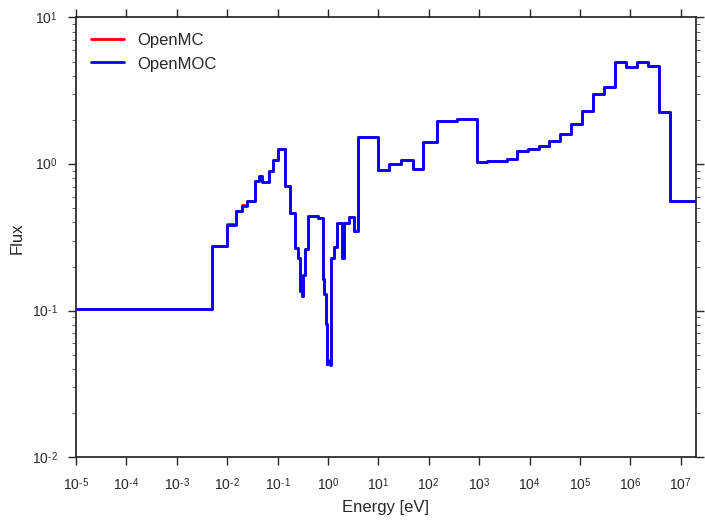
\includegraphics[width=0.8\linewidth]{figures/biases/slab/vol-avg-flux}
\caption[Flux spectrum in a 1D slab.]{The normalized volume-weighted flux spectrum in energy in a 1D slab.}
\label{fig:chap4-slab-flux}
\end{figure}

\begin{figure}[H]
  \centering
  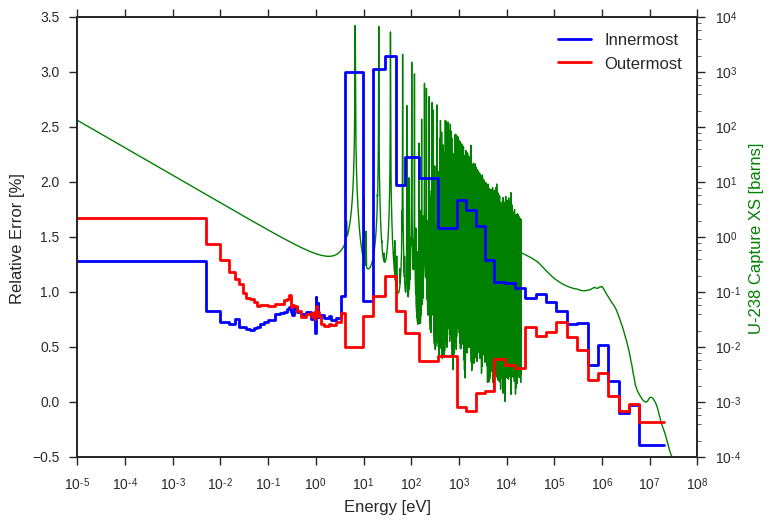
\includegraphics[width=0.85\linewidth]{figures/biases/slab/rel-err-inner-outer}
\caption[Flux relative error by group for a 1D slab.]{The relative error of the OpenMOC scalar flux with respect to the reference OpenMC flux. The errors are illustrated for the innermost and outermost fuel \ac{FSR}s of the 16$\times$ discretization case along with the U-238 capture cross section.}
\label{fig:chap4-slab-rel-err}
\end{figure}

\begin{figure}[H]
  \centering
  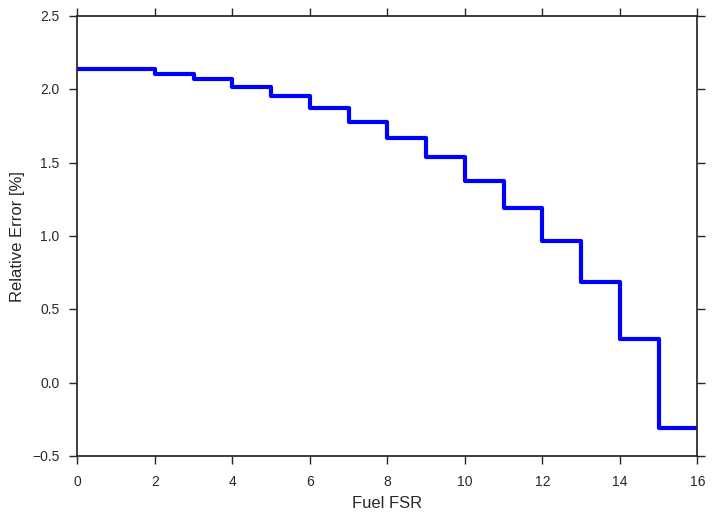
\includegraphics[width=0.85\linewidth]{figures/biases/slab/rel-err-fuel-fsrs}
\caption[Flux relative error by fuel FSR for a 1D slab.]{The relative error of the OpenMOC scalar flux with respect to the reference OpenMC flux. The errors are plotted for each fuel \ac{FSR} in the 16$\times$ discretization case.}
\label{fig:chap4-slab-fuel-fsrs}
\end{figure}


%\begin{figure}[h!]
%  \centering
%  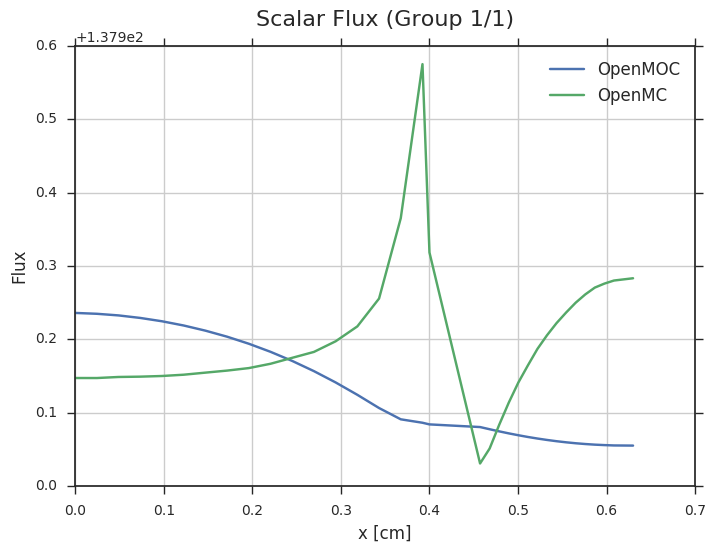
\includegraphics[width=0.9\linewidth]{figures/biases/slab/flux-group-1-1}
%  \caption{}
%\label{fig:chap2-slab-flux}
%\caption[Spatially-varying scalar flux a 1D slab.]{The volume-averaged reference OpenMC flux and OpenMOC flux computed with 70-group spatially-varying \ac{MGXS} in the fuel.}
%\end{figure}

%\begin{figure}[H]
%\begin{subfigure}{\linewidth}
%  \centering
%  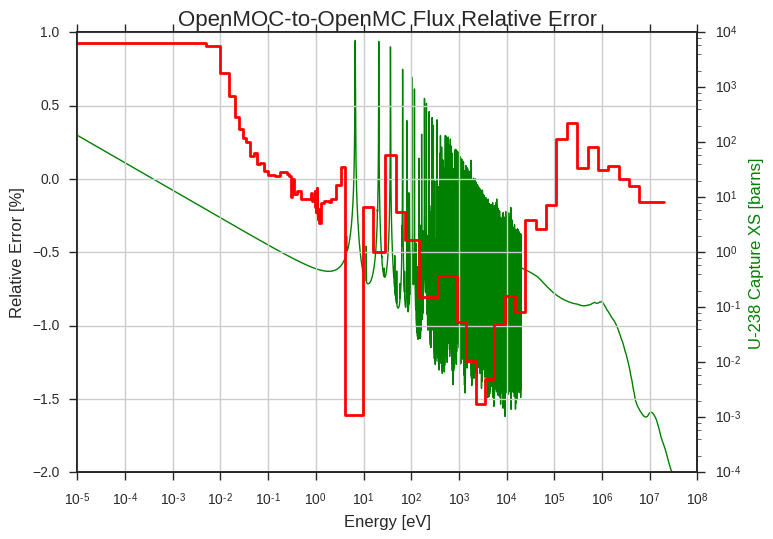
\includegraphics[width=0.9\linewidth]{figures/biases/slab/rel-err-fuel-inner}
%  \caption{}
%\end{subfigure}
%\begin{subfigure}{\linewidth}
%  \centering
%  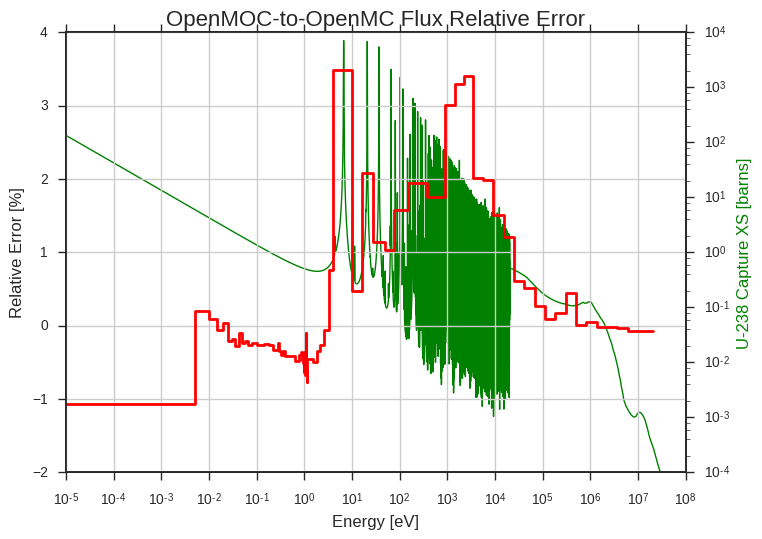
\includegraphics[width=0.9\linewidth]{figures/biases/slab/rel-err-fuel-outer}
%  \caption{}
%\end{subfigure}
%\label{fig:chap4-slab-rel-err}
%\caption[Flux relative error by group for a 1D slab.]{The percent relative error of the OpenMOC scalar flux with respect to the tallied reference OpenMC flux spectrum. The flux errors are illustrated by energy group for the innermost (a) and outermost (b) \ac{FSR}s of the 16$\times$ discretization case.}
%\end{figure}


%%%%%%%%%%%%%%%%%%%%%%%%%%%%%
\subsection{2D Fuel Pin Cell}
\label{subsec:chap4-pin}

A \ac{PWR} fuel pin cell model was constructed to quantify approximation errors in a 2D heterogeneous geometry with spatial self-shielding. The pin cell is identical to the 1.6\% enriched UO$_2$ \ac{PWR} fuel pin in the \ac{BEAVRS} \ac{PWR} model~\cite{horelik2013beavrs}. The geometric configuration of UO$_2$ fuel, helium gap, zirconium clad and water moderator is illustrated in Figure~\ref{fig:chap4-pin-cell} and the dimensions for each material zone are shown in Table~\ref{table:chap2-pin-dimensions}. Reflective boundary conditions were applied to all edges in the geometry. The isotopic compositions of each material in the fuel pin were identical to those used in the 1D slab and are itemized in Table~\ref{table:chap2-slab-isotopes}. 

\begin{figure}[H]
\centering
\begin{subfigure}{.32\textwidth}
  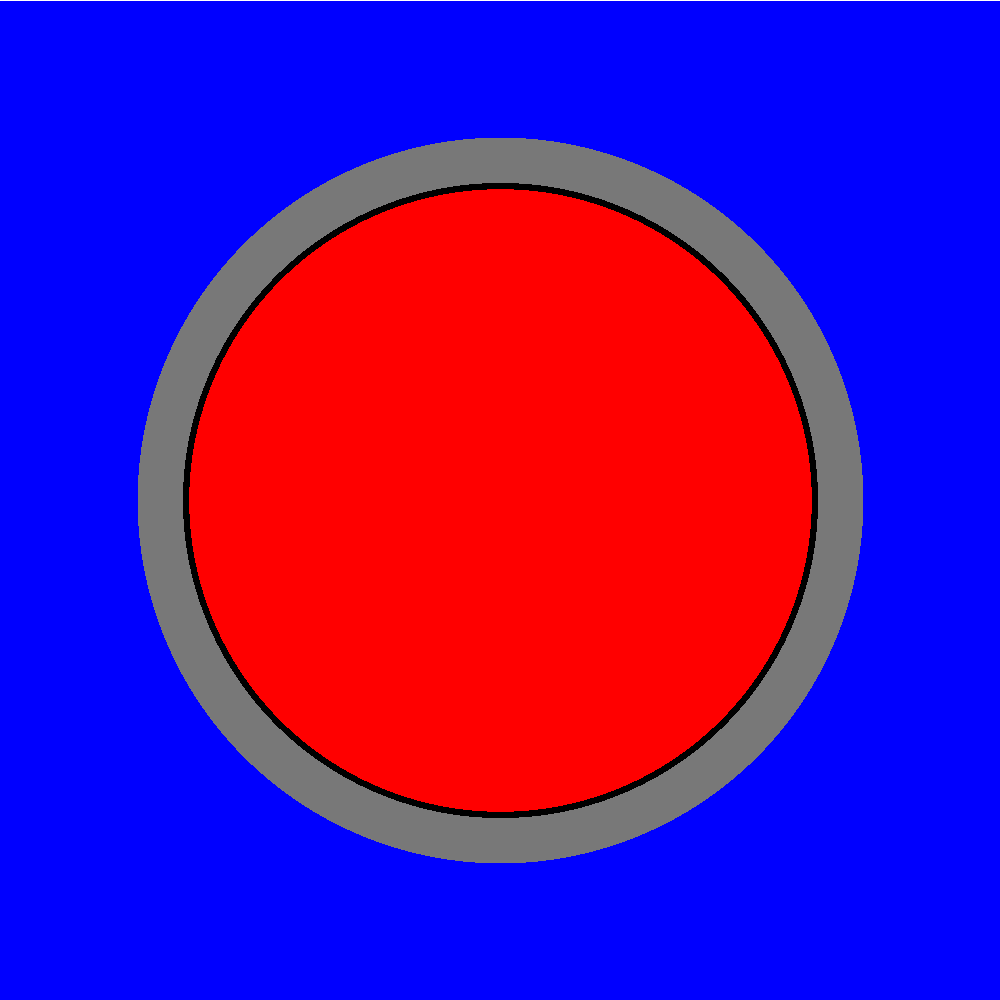
\includegraphics[width=0.9\linewidth]{figures/biases/pin-cell/pin-cell-simple}
  \caption{}
\end{subfigure}%
\begin{subfigure}{.32\textwidth}
  \centering
  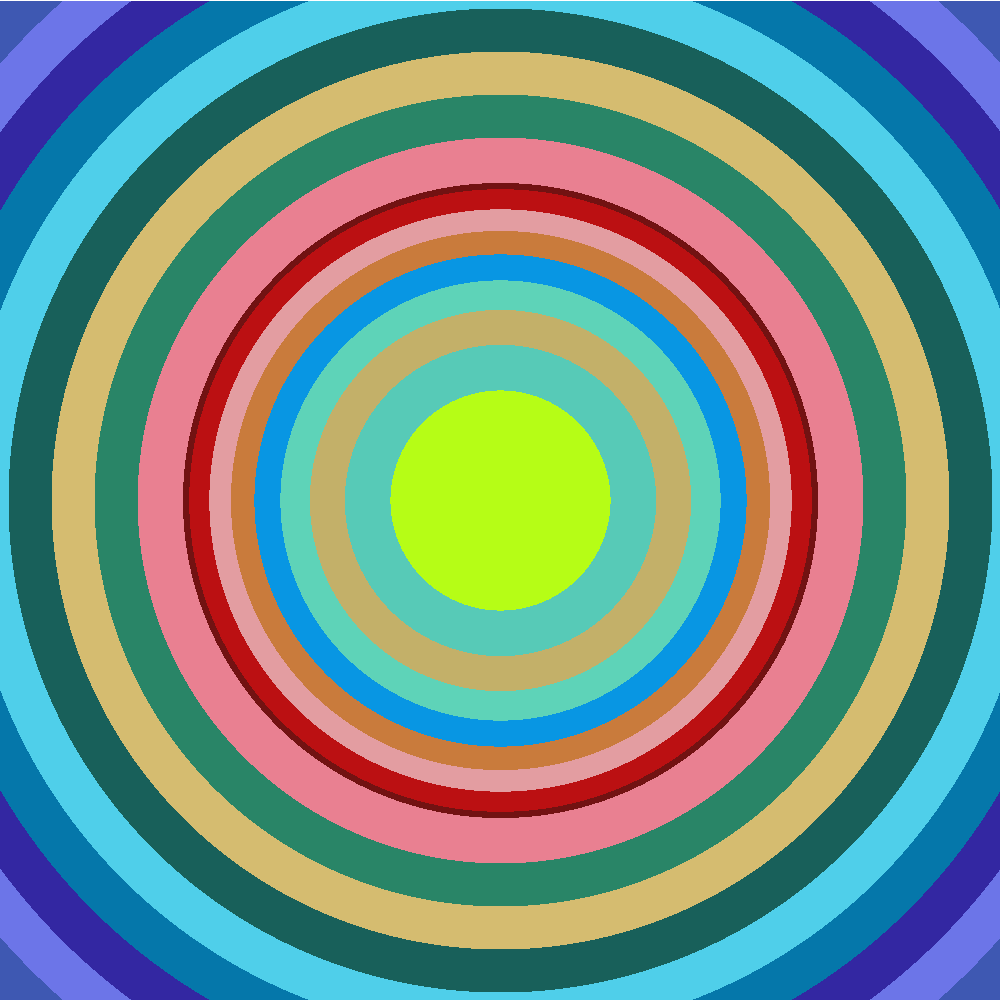
\includegraphics[width=0.9\linewidth]{figures/biases/pin-cell/pin-cell-8x}
  \caption{}
\end{subfigure}
\begin{subfigure}{.32\textwidth}
  \centering
  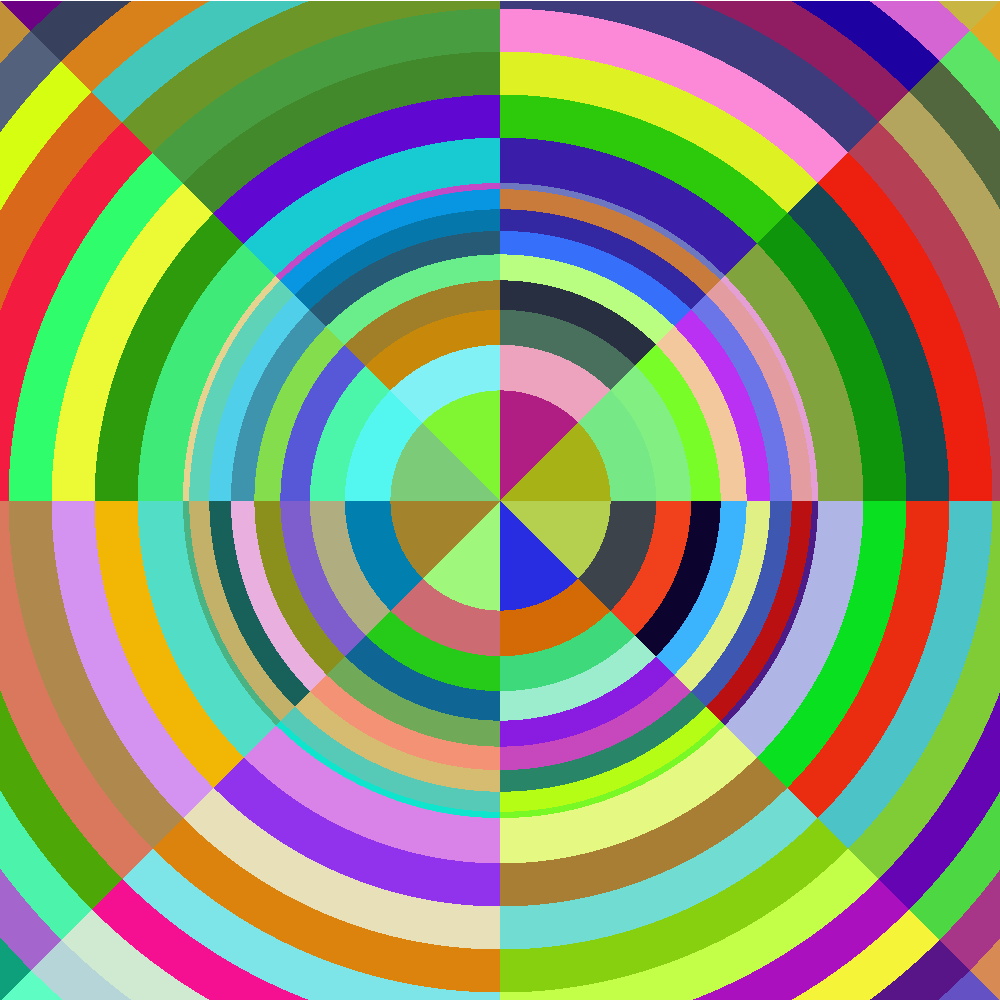
\includegraphics[width=0.9\linewidth]{figures/biases/pin-cell/pin-cell-8x8}
  \caption{}
\end{subfigure}
\caption[Pin cell materials and geometry]{A PWR fuel pin cell with fuel, gap, clad and moderator (a). Radial tally zones were defined in each material in OpenMC (b). The tally zones were further subdivided into angular sectors for the \ac{FSR} mesh in OpenMOC (c).}
\label{fig:chap4-pin-cell}
\end{figure}

\begin{table}[h!]
  \centering
  \caption{2D fuel pin dimensions.}
  \label{table:chap2-pin-dimensions} 
  \vspace{6pt}
  \begin{tabular}{l c}
  \toprule
  \multicolumn{1}{c}{\bf Material} &
  \multicolumn{1}{c}{\bf Dimension [cm]} \\
  \midrule
  Fuel Outer Radius &     0.39218 \\
  Gap Outer Radius &      0.40005 \\
  Clad Outer Radius &     0.45720 \\
  Pin Pitch &             1.25984 \\
  \bottomrule
\end{tabular}
\end{table}

%\begin{table}[h!]
%  \centering
%  \caption{2D fuel pin isotopic composition.}
%  \label{table:chap2-pin-isotopes} 
%  \vspace{6pt}
%  \begin{tabular}{l c c}
%  \toprule
%  \multicolumn{1}{c}{\bf Material} &
%  \multicolumn{1}{c}{\bf Nuclide} &
%  \multicolumn{1}{c}{\bf Atom Density [at/b-cm]} \\
%  \midrule
%  \multirow{3}{*}{\bf UO$_2$} & O-16 &  4.5850826385693E-2 \\
%  & U-235 & 5.5841582288888E-4 \\
%  & U-238 & 2.2418671968636E-2 \\
%  \midrule
%  \multirow{1}{*}{\bf Helium} & He-4 & 2.40428068880973E-4 \\
%  \midrule
%  \multirow{3}{*}{\bf Zircaloy} & O-16 &  6.1404143720635E-4 \\
%  & Fe-56 & 2.7183762028359E-4 \\
%  & Zr-90 & 4.3595883452828E-2 \\
%  \midrule
%  \multirow{4}{*}{\bf Water} & H-1 &  4.95774559287053E-2 \\
%  & B-10 & 8.02369478020388E-6 \\
%  & B-11 & 3.22964691572685E-5 \\
%  & O-16 & 2.47320903547125E-2 \\
%  \bottomrule
%\end{tabular}
%\end{table}

The reference eigenvalues computed with continuous energy cross sections in OpenMC are shown in Table~\ref{table:chap2-pin-reference} for both normal anisotropic as well as ``iso-in-lab'' scattering. The reference calculations were computed for 100 batches of 1E7 particles per batch. The reference eigenvalues for the two cases vary by roughly 65 pcm, slightly more than in the 1D slab geometry. The \texttt{openc.mgxs} module was used to compute 70-group libraries of $\Sigma^T_g$, $\Sigma^{Tr}_g$, $\nu\Sigma^F_g$, $\nu_s\Sigma^S_{gg'}$ and $\chi_g$ from OpenMC tallies. An installation of OpenMOC compiled with double precision floating point arithmetic was used for each deterministic simulation. In each calculation, OpenMOC was converged to a criterion of 1E-7 on the energy-integrated fission source.

\begin{table}[h!]
  \centering
  \caption{Reference $k^{OpenMC}_{eff}$ for an 2D fuel pin.}
  \label{table:chap2-pin-reference} 
  \vspace{6pt}
  \begin{tabular}{c c}
  \toprule
  \multicolumn{1}{c}{\bf Anisotropic} &
  \multicolumn{1}{c}{\bf Isotropic in Lab} \\
  \midrule
  1.17486 $\pm$ 0.00003 & 1.17421 $\pm$ 0.00002 \\
  \bottomrule
\end{tabular}
\end{table}

Table~\ref{table:chap2-pin-angle} presents the bias $\Delta\rho$ for a matrix of azimuthal angles and track spacings. No transport correction was applied to the total cross section $\Sigma^T_g$ or the scattering matrix $\nu_s\Sigma^S_{gg'}$. Each of the material zones was discretized into 8 angular sectors for the \ac{FSR} mesh in OpenMOC. The results for both normal anisotropic scattering and ``iso-in-lab'' scattering exhibit a bias of a few hundred pcm or less depending on the energy and spatial mesh. The magnitude of the bias appears to converge with 128 azimuthal angles and is largely invariant with the track spacing. The \ac{MGXS} tallied with ``iso-in-lab'' scattering in OpenMC converge to an eigenvalue that is roughly 40 pcm less than that computed for the anisotropic case, with a bias of approximately -30 pcm.

\begin{table}[h!]
  \centering
  \caption[Angular discretization error for a 2D fuel pin]{Convergence study of the eigenvalue bias $\Delta\rho$ with varying azimuthal angle quadratures and track spacings for a 2D fuel pin.}
  \label{table:chap2-pin-angle}
  \vspace{6pt}
  \begin{tabular}{c S[table-format=2.1] S[table-format=2.1] S[table-format=2.1] c S[table-format=2.1] S[table-format=2.1] S[table-format=2.1]} 
  \toprule
  & \multicolumn{7}{c}{\boldmath $\Delta\rho$ {\bf [pcm]}} \\
  \midrule
  \multicolumn{1}{c}{\bf \# Angles} &
  \multicolumn{1}{c}{\bf 0.1 cm} & 
  \multicolumn{1}{c}{\bf 0.01 cm} & 
  \multicolumn{1}{c}{\bf 0.001 cm} &
  \multicolumn{1}{c}{} &
  \multicolumn{1}{c}{\bf 0.1 cm} & 
  \multicolumn{1}{c}{\bf 0.01 cm} & 
  \multicolumn{1}{c}{\bf 0.001 cm} \\
  \midrule
  & \multicolumn{3}{c}{\bf Anisotropic} &
  \multicolumn{1}{c}{} &
  \multicolumn{3}{c}{\bf Isotropic in Lab} \\
  \cline{2-4} \cline{6-8}
4 & 365 & 390 & 391 & & 460 & 484 & 486 \\
8 & -251 & -289 & -285 & & -157 & -194 & -191 \\
16 & -297 & -263 & -266 & & -202 & -168 & -171 \\
32 & -180 & -196 & -188 & & -86 & -101 & -94 \\
64 & -112 & -154 & -143 & & -18 & -60 & -49 \\
128 & -139 & -134 & -125 & & -45 & -39 & -31 \\
256 & -131 & -125 & -123 & & -36 & -30 & -28 \\
512 & -124 & -121 & -122 & & -30 & -27 & -28 \\
  \bottomrule
\end{tabular}
\end{table}

Table~\ref{table:chap2-pin-energy} presents the bias $\Delta\rho$ between OpenMC and OpenMOC for a matrix of energy group structures and \ac{FSR} spatial discretizations. In each case, the \ac{MGXS} used in OpenMOC were tallied by material in OpenMC. The OpenMOC calculations each used 128 azimuthal angles and 0.05 cm track spacing. Each of the materials in the fuel pin was radially discretized into 1 -- 16 equal volume rings. 

\begin{table}[h!]
  \centering
  \caption[Energy and spatial discretization error for a 2D fuel pin]{Convergence study of the eigenvalue bias $\Delta\rho$ with varying energy groups structures and \ac{FSR} spatial discretizations for a 2D fuel pin with \ac{MGXS} tallied by material.}
  \label{table:chap2-pin-energy} 
  \vspace{6pt}
  \begin{tabular}{c S[table-format=6.1] S[table-format=6.1] S[table-format=6.1] S[table-format=6.1] S[table-format=6.1]}
  \toprule
  & \multicolumn{5}{c}{\boldmath $\Delta\rho$ {\bf [pcm]}} \\
  \midrule  
  \multicolumn{1}{c}{\textbf{\# Groups}} &
  \multicolumn{1}{c}{\bf 1$\times$} &
  \multicolumn{1}{c}{\bf 2$\times$} &
  \multicolumn{1}{c}{\bf 4$\times$} &
  \multicolumn{1}{c}{\bf 8$\times$} &
  \multicolumn{1}{c}{\bf 16$\times$} \\
  \midrule
  & \multicolumn{5}{c}{\bf Anisotropic $\left(\Sigma^T_g\right)$} \\
  \cline{2-6}
1 & 77 & 78 & 78 & 78 & 78 \\
2 & 34 & -10 & -40 & -52 & -50 \\
4 & -55 & -95 & -123 & -137 & -145 \\
8 & -71 & -131 & -177 & -198 & -208 \\
16 & -68 & -135 & -188 & -212 & -223 \\
25 & -126 & -189 & -241 & -267 & -275 \\
40 & -129 & -197 & -253 & -282 & -290 \\
70 & -129 & -200 & -259 & -289 & -298 \\
  \cline{2-6}
  & \multicolumn{5}{c}{\bf Anisotropic $\left(\Sigma^{Tr}_g\right)$} \\
  \cline{2-6}
1 & 63 & 64 & 64 & 64 & 63 \\
2 & 52 & 22 & 4 & -2 & 6 \\
4 & -60 & -89 & -108 & -125 & -126 \\
8 & -75 & -123 & -157 & -180 & -183 \\
16 & -68 & -123 & -165 & -191 & -194 \\
25 & -128 & -182 & -225 & -250 & -253 \\
40 & -133 & -192 & -241 & -268 & -272 \\
70 & -135 & -196 & -248 & -277 & -281 \\
  \cline{2-6}
  & \multicolumn{5}{c}{\bf Isotropic in Lab $\left(\Sigma^T_g\right)$} \\
  \cline{2-6}
1 & 91 & 92 & 92 & 93 & 92 \\
2 & 153 & 109 & 78 & 67 & 69 \\
4 & 31 & -9 & -38 & -51 & -59 \\
8 & 31 & -29 & -75 & -95 & -106 \\
16 & 41 & -26 & -79 & -103 & -114 \\
25 & -27 & -91 & -142 & -169 & -177 \\
40 & -34 & -103 & -159 & -187 & -196 \\
70 & -35 & -106 & -165 & -195 & -204 \\
  \bottomrule
\end{tabular}
\end{table}

The results indicate a strong interaction between the energy and spatial discretization, as the eigenvalue bias exhibits a swing of nearly 10000-15000 pcm between energy and spatial meshes. The application of the P0 transport correction has a marked impact in reducing the bias if and only if fine energy and spatial meshes are simultaneously utilized. The results with OpenMC's ``iso-in-lab'' scattering feature similarly point to the need for both a fine energy and spatial mesh to minimize and converge the bias from the multi-group approximation.

-mention angular discretization \\

Table~\ref{table:chap2-pin-space} presents the bias $\Delta\rho$ for a matrix of energy group structures and \ac{MGXS} spatial tally zone meshes. In each case, the \ac{MGXS} were tallied in the \ac{FSR} mesh used in OpenMOC with 1 -- 16 equal volume rings per material. The OpenMOC calculations each used 128 azimuthal angles and 0.05 cm track spacing.

\begin{table}[h!]
  \centering
  \caption[Spatial homogenization error for a 2D fuel pin]{Convergence study of the eigenvalue bias $\Delta\rho$ with varying energy groups structures and \ac{FSR} spatial discretizations for a 2D fuel pin with \ac{MGXS} tallied by \ac{FSR}.}
  \label{table:chap2-pin-space} 
  \vspace{6pt}
  \begin{tabular}{c S[table-format=6.1] S[table-format=6.1] S[table-format=6.1] S[table-format=6.1] S[table-format=6.1]}
  \toprule
  & \multicolumn{5}{c}{\boldmath $\Delta\rho$ {\bf [pcm]}} \\
  \midrule  
  \multicolumn{1}{c}{\textbf{\# Groups}} &
  \multicolumn{1}{c}{\bf 1$\times$} &
  \multicolumn{1}{c}{\bf 2$\times$} &
  \multicolumn{1}{c}{\bf 4$\times$} &
  \multicolumn{1}{c}{\bf 8$\times$} &
  \multicolumn{1}{c}{\bf 16$\times$} \\
  \midrule
  & \multicolumn{5}{c}{\bf Anisotropic $\left(\Sigma^T_g\right)$} \\
  \cline{2-6}
 & 79 & 78 & 62 & 62 & 53 \\
2 & 36 & -7 & -57 & -93 & -92 \\
4 & -53 & -90 & -136 & -173 & -184 \\
8 & -70 & -127 & -190 & -240 & -247 \\
16 & -66 & -130 & -198 & -255 & -257 \\
25 & -124 & -189 & -257 & -321 & -324 \\
40 & -127 & -200 & -272 & -339 & -344 \\
70 & -128 & -204 & -278 & -347 & -353 \\
  \cline{2-6}
  & \multicolumn{5}{c}{\bf Anisotropic $\left(\Sigma^{Tr}_g\right)$} \\
  \cline{2-6}
1 & 65 & 79 & 74 & 30 & 33 \\
2 & 54 & 34 & 4 & -45 & -33 \\
4 & -58 & -77 & -106 & -166 & -165 \\
8 & -73 & -111 & -159 & -227 & -227 \\
16 & -66 & -111 & -168 & -238 & -240 \\
25 & -126 & -178 & -238 & -310 & -310 \\
40 & -131 & -188 & -256 & -330 & -331 \\
70 & -133 & -193 & -263 & -339 & -340 \\
  \cline{2-6}
  & \multicolumn{5}{c}{\bf Isotropic in Lab $\left(\Sigma^T_g\right)$} \\
  \cline{2-6}
1 & 92 & 109 & 54 & 48 & 28 \\
2 & 154 & 107 & 28 & 12 & -6 \\
4 & 32 & -3 & -52 & -91 & -107 \\
8 & 32 & -22 & -93 & -136 & -152 \\
16 & 42 & -23 & -99 & -147 & -161 \\
25 & -26 & -95 & -169 & -220 & -238 \\
40 & -33 & -104 & -186 & -241 & -259 \\
70 & -34 & -107 & -193 & -247 & -267 \\
  \bottomrule
\end{tabular}
\end{table}

\begin{itemize}
  \item rework writeup
  \item 70-group flux
  \item compare 70-group flux errors with U-238 capture XS - volume-avg
  \item compare 70-group flux errors with U-238 capture XS - fuel mesh zone nearest clad
\end{itemize}

\begin{figure}[h!]
  \centering
  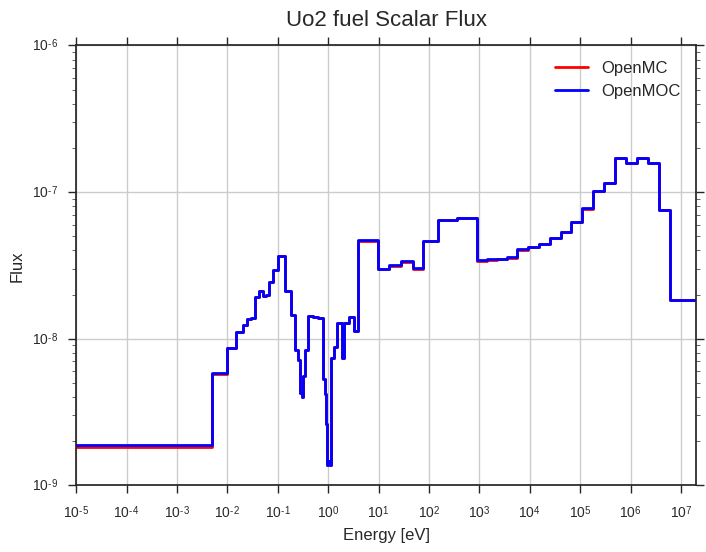
\includegraphics[width=0.9\linewidth]{figures/biases/pin-cell/flux-uo2-fuel}
\caption[Spatially-varying scalar flux a 2D fuel pin.]{The volume-averaged reference OpenMC flux and OpenMOC flux computed with 70-group spatially-varying \ac{MGXS} in the fuel.}
\label{fig:chap2-pin-flux}
\end{figure}

\begin{figure}[h!]
\begin{subfigure}{\linewidth}
  \centering
  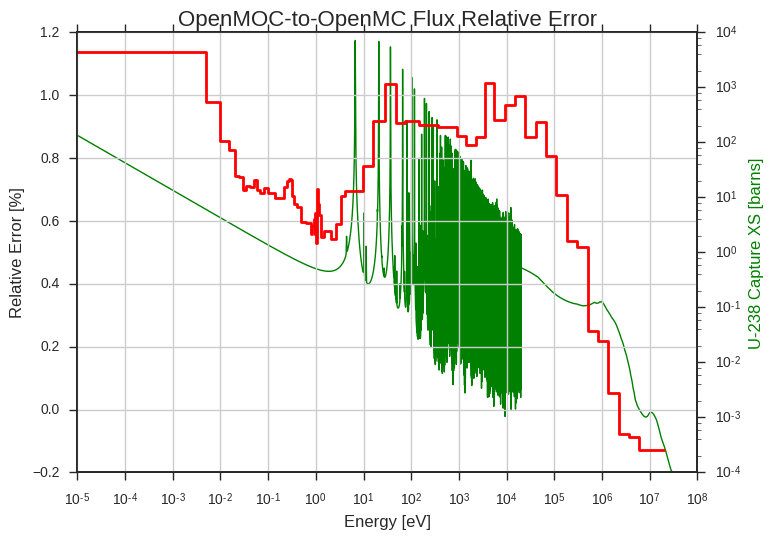
\includegraphics[width=0.9\linewidth]{figures/biases/pin-cell/rel-err-fuel-inner}
  \caption{}
\end{subfigure}
\begin{subfigure}{\linewidth}
  \centering
  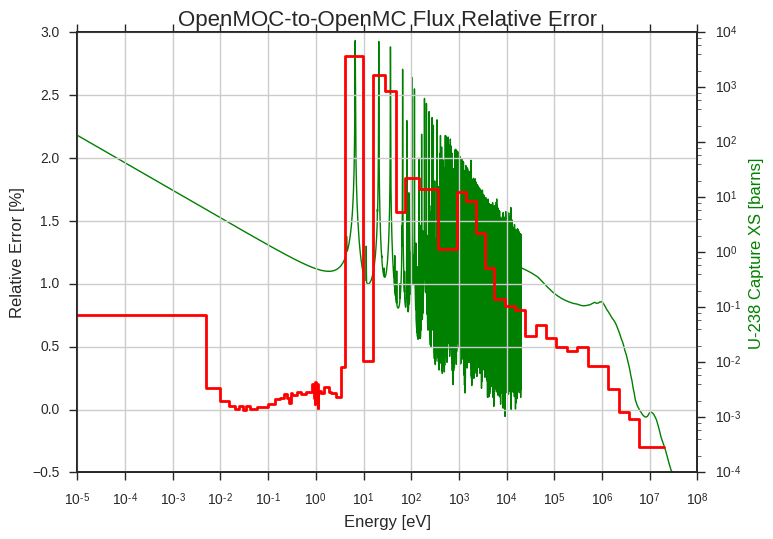
\includegraphics[width=0.9\linewidth]{figures/biases/pin-cell/rel-err-fuel-outer}
  \caption{}
\end{subfigure}
\label{fig:chap2-pin-rel-err}
\caption[Flux relative error by group for a 2D fuel pin.]{The percent relative error of the OpenMOC scalar flux with respect to the reference OpenMOC flux spectrum. The flux errors are illustrated by energy group for the innermost (a) and outermost (b) rings of the 16$\times$ discretization case.}
\end{figure}


%%%%%%%%%%%%%%%%%%%%%%%%%%%%%%%%%%%%%%%%%%%
%\subsection{2D Fuel Assembly}
